\documentclass{ximera}
\begin{document}

    \title{Lecture 4}
    
    \begin{abstract} 
    - Condition numbers of matrices \\
    - Vector and matrix norms \\
    \end{abstract}
    \maketitle

\textit{Most (not all) of this lecture corresponds to Lecture 3 in your textbook}

\vspace{0.1in}

Suppose I am considering the problem that this entire class is about: $Ax = b$.  Numerically, I will have some trouble potentially representing $A$ and $b$, so maybe my computer will actually be solving the problem $(A+\delta A) \hat{x} = b+\delta b$.  We want to bound the norm of the error $\delta x:= \hat{x} - x$.  Let's do a simple subtraction:

\begin{align*}
    (A+\delta A)(x+\delta x) &= b+ \delta b \\
    - \phantom{yoooomannnnn} Ax&=b\\
    \hline
    \delta Ax + (A+\delta A)\delta x &= \delta b
\end{align*}
Rearranging yields
\begin{align}
    \delta x = A^{-1}(-\delta A\hat{x} + \delta b).
\end{align}

Taking norms, we see that 
\begin{align}
    \|\delta x\| = \|A^{-1}(-\delta A\hat{x} + \delta b)\|.
\end{align}
Right now, I am having trouble understanding how this norm relates to the structure of $A^{-1}$ and $\delta A$ in general, as well as $\delta b$ and $\hat{x}$, because the norm is on the whole product.  Let's use this to motivate looking at a more general definition of norms of vectors, and also norms of matrices (also known as an operator norm).

\begin{definition}
    A norm is a function $\|\cdot \|: \mathbb{C}^m \to \mathbb{R}$ that assigns a real-valued length to each vector.  It satisfies the following three conditions: for all $x, y \in \mathbb{C}^m$ and for all $\alpha \in \mathbb{C}$,
    \begin{enumerate}
        \item $\|x\|\geq 0$, and $\|x\| = 0$ only if $x=0$
        \item $\|x+y\| \leq \|x\| + \|y\|$
        \item $\|\alpha x\| = |\alpha|\|x\|$.
    \end{enumerate}
\end{definition}

Before, we mentioned only the Euclidean norm; this is the more general definition of norm, giving us a lot of flexibility in assigning new types of lengths (e.g., yards vs meters).

The most important class of vector norms, the $p$-norms, are defined with images below:

\begin{center}
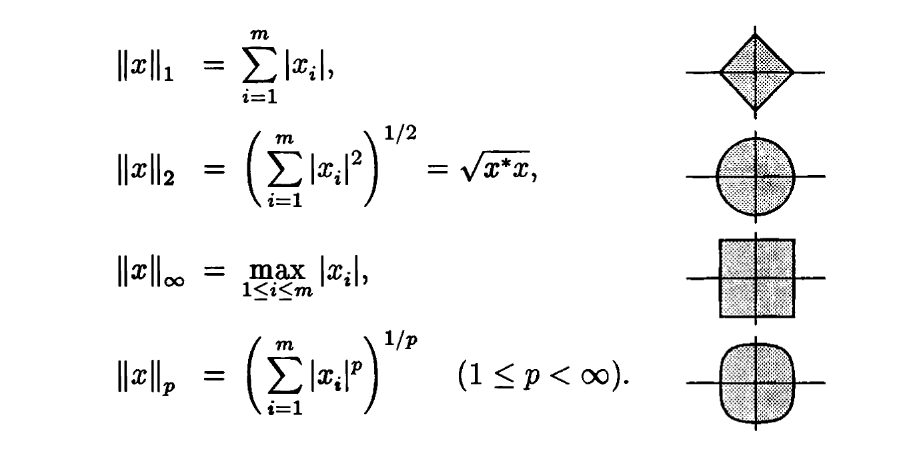
\includegraphics[width=0.85\textwidth]{xmPictures/norms_pic.png}
\end{center}

Weighted $p$-norms: $\|x\|_W = \|Wx\|$ for some $W$ a diagonal matrix where the $i$th diagonal entry is the weight $w_i\neq 0$.  

\begin{center}
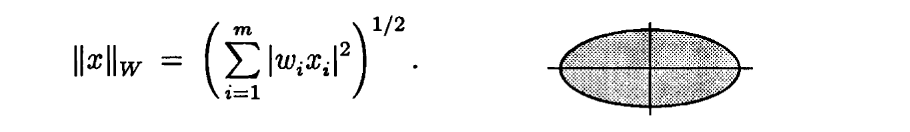
\includegraphics[width=0.85\textwidth]{xmPictures/weighted_2norm.png}
\end{center}

Matrices are operators, specifically linear transformations.  You can think about them as vectors in different spaces (which is in fact how your computer stores matrices), and consequently they also can have norms.  In fact, more generally, they have operator norms, defined in the following manner:
\begin{definition}
    Let $A \in \mathbb{C}^{m\times n}$.  Given some vector norms $\|\cdot \|_{(n)}$ on $\mathbb{C}^n$ (the domain of $A$) and $\|\cdot\|_{(m)}$ on $\mathbb{C}^m$ (the range of $A$), the induced matrix norm is the smallest number $C$ such that
    \begin{align*}
        \|Ax\|_{(m)} \leq C \|x\|_{(n)}.
    \end{align*}
    Rearranging, this can be rewritten so that 
    \begin{align*}
        \|A\|_{(m,n)} = \sup\limits_{\stackrel{x \in \mathbb{C}^n}{x\neq 0}}  \frac{\|Ax\|_{(m)}}{\|x\|_{(n)}} = \sup\limits_{\stackrel{x \in \mathbb{C}^n}{x\neq 0}}  \left\|A\frac{x}{\|x\|_{(n)}}\right\|_{(m)} \\
        = \sup\limits_{\stackrel{x \in \mathbb{C}^n}{\|x\|_{(n)}=1}} \|Ax\|_{(m)}
    \end{align*}
\end{definition}

There is an equivalent formulation of this norm, specifically, 
\begin{align*}
    \sup\limits_{\stackrel{x \in \mathbb{C}^n}{\|x\|_{(n)}=1}} \|Ax\|_{(m)} = \sup\limits_{\stackrel{x \in \mathbb{C}^n}{\|x\|_{(n)}\leq 1}} \frac{\|Ax\|_{(m)}}{\|x\|_{(n)}}
\end{align*}
Clearly, 
\begin{align*}
    \sup\limits_{\stackrel{x \in \mathbb{C}^n}{\|x\|_{(n)}=1}} \|Ax\|_{(m)} \leq \sup\limits_{\stackrel{x \in \mathbb{C}^n}{\|x\|_{(n)}\leq 1}}\frac{\|Ax\|_{(m)}}{\|x\|_{(n)}}, 
\end{align*}
since the admissible set of solutions is larger on the right hand side (the candidates are pulled from the set $\|x\| \leq 1$ instead of $\|x\| = 1$).  Moreover,  
\begin{align*}
    \sup\limits_{\stackrel{x \in \mathbb{C}^n}{\|x\|_{(n)}\leq 1}}\frac{\|Ax\|_{(m)}}{\|x\|_{(n)}} \leq \sup\limits_{\stackrel{x \in \mathbb{C}^n}{x\neq 0}}  \frac{\|Ax\|_{(m)}}{\|x\|_{(n)}},
\end{align*}
again since the admissible set on the right hand side of the inequality is larger than that on the left hand side.  Thus, 
\begin{align*}
    \sup\limits_{\stackrel{x \in \mathbb{C}^n}{\|x\|_{(n)}=1}} \|Ax\|_{(m)} \leq \sup\limits_{\stackrel{x \in \mathbb{C}^n}{\|x\|_{(n)}\leq 1}}\frac{\|Ax\|_{(m)}}{\|x\|_{(n)}}
    \leq
    \sup\limits_{\stackrel{x \in \mathbb{C}^n}{x\neq 0}}  \frac{\|Ax\|_{(m)}}{\|x\|_{(n)}}.
\end{align*}
Since the upper bound equals the lower bound, it is in fact true that 
\begin{align*}
    \sup\limits_{\stackrel{x \in \mathbb{C}^n}{\|x\|_{(n)}=1}} \|Ax\|_{(m)} = \sup\limits_{\stackrel{x \in \mathbb{C}^n}{\|x\|_{(n)}\leq 1}}\frac{\|Ax\|_{(m)}}{\|x\|_{(n)}}
    =
    \sup\limits_{\stackrel{x \in \mathbb{C}^n}{x\neq 0}}  \frac{\|Ax\|_{(m)}}{\|x\|_{(n)}}.
\end{align*}

\begin{example}
    Consider $A = \begin{bmatrix} 1 &2 \\ 0 & 2\end{bmatrix}$.
    To understand the induced matrix norm of $A$, we look at how $A$ transforms the geometric shapes for the vectors in the unit ball of choice in the domain.  For example, how does $A$ transform the diamond-shaped unit ball of the $1$-norm?  the circular shaped ball of the $2$-norm?  the square-shaped ball of the $\infty$-norm.
\end{example}

\begin{center}
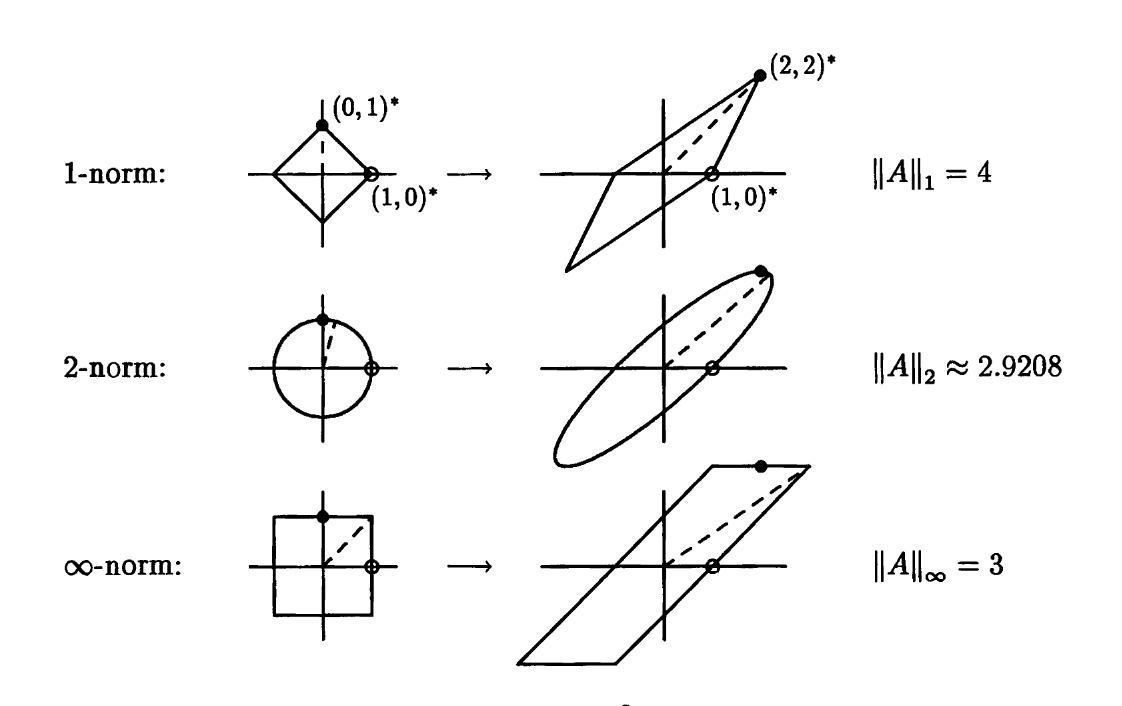
\includegraphics[width=0.85\textwidth]{xmPictures/Atransforms_unitBalls.png}
\end{center}

\end{document}



